\documentclass{beamer}\usepackage[]{graphicx}\usepackage[]{color}
%% maxwidth is the original width if it is less than linewidth
%% otherwise use linewidth (to make sure the graphics do not exceed the margin)
\makeatletter
\def\maxwidth{ %
  \ifdim\Gin@nat@width>\linewidth
    \linewidth
  \else
    \Gin@nat@width
  \fi
}
\makeatother

\definecolor{fgcolor}{rgb}{0.345, 0.345, 0.345}
\newcommand{\hlnum}[1]{\textcolor[rgb]{0.686,0.059,0.569}{#1}}%
\newcommand{\hlstr}[1]{\textcolor[rgb]{0.192,0.494,0.8}{#1}}%
\newcommand{\hlcom}[1]{\textcolor[rgb]{0.678,0.584,0.686}{\textit{#1}}}%
\newcommand{\hlopt}[1]{\textcolor[rgb]{0,0,0}{#1}}%
\newcommand{\hlstd}[1]{\textcolor[rgb]{0.345,0.345,0.345}{#1}}%
\newcommand{\hlkwa}[1]{\textcolor[rgb]{0.161,0.373,0.58}{\textbf{#1}}}%
\newcommand{\hlkwb}[1]{\textcolor[rgb]{0.69,0.353,0.396}{#1}}%
\newcommand{\hlkwc}[1]{\textcolor[rgb]{0.333,0.667,0.333}{#1}}%
\newcommand{\hlkwd}[1]{\textcolor[rgb]{0.737,0.353,0.396}{\textbf{#1}}}%
\let\hlipl\hlkwb

\usepackage{framed}
\makeatletter
\newenvironment{kframe}{%
 \def\at@end@of@kframe{}%
 \ifinner\ifhmode%
  \def\at@end@of@kframe{\end{minipage}}%
  \begin{minipage}{\columnwidth}%
 \fi\fi%
 \def\FrameCommand##1{\hskip\@totalleftmargin \hskip-\fboxsep
 \colorbox{shadecolor}{##1}\hskip-\fboxsep
     % There is no \\@totalrightmargin, so:
     \hskip-\linewidth \hskip-\@totalleftmargin \hskip\columnwidth}%
 \MakeFramed {\advance\hsize-\width
   \@totalleftmargin\z@ \linewidth\hsize
   \@setminipage}}%
 {\par\unskip\endMakeFramed%
 \at@end@of@kframe}
\makeatother

\definecolor{shadecolor}{rgb}{.97, .97, .97}
\definecolor{messagecolor}{rgb}{0, 0, 0}
\definecolor{warningcolor}{rgb}{1, 0, 1}
\definecolor{errorcolor}{rgb}{1, 0, 0}
\newenvironment{knitrout}{}{} % an empty environment to be redefined in TeX

\usepackage{alltt}

\usepackage{default}
\usepackage{animate} %need the animate.sty file 
\usepackage{graphicx}
%\graphicspath{{/home/sahir/Dropbox/jobs/laval/minicours/slides/}}
\usepackage{hyperref, url}
%\usepackage[round,sort]{natbib}   % bibliography omit 'round' option if you prefer square brackets
%\bibliographystyle{apalike}
\usepackage{biblatex}
\bibliography{bib.bib}
% Removes icon in bibliography
\setbeamertemplate{bibliography item}[text]

\usepackage[normalem]{ulem}

\setbeamertemplate{theorems}[numbered]



%\newtheorem{prop}{Proposition}
%\newenvironment{theoremc}[1]
%{\begin{shaded}\begin{theorem}[#1]}
%		{\end{theorem}\end{shaded}}
	
%\newtheorem{examplefirst}{Example}
%\newtheorem{examplesecond}{Example}
%\newenvironment<>{examplefirst}[1][]{%
%	\setbeamercolor{block title example}{bg=lightgray}%
%	\begin{example}#2[#1]}{\end{example}}
%\newenvironment<>{examplesecond}[1][]{%
%	\setbeamercolor{block title example}{fg=white,bg=blue!75!black}%
%	\begin{example}#2[#1]}{\end{example}}	

%\usepackage{amsthm}


\usepackage[figurename=Fig.]{caption}
\usepackage{subfig}
\usepackage{tikz, pgfplots,epsfig}
\usetikzlibrary{arrows,shapes.geometric}
\usepackage{color, colortbl,xcolor}
\definecolor{lightgray}{RGB}{200,200,200}
\definecolor{palegray}{RGB}{221,221,221}
\definecolor{myblue}{RGB}{0,89,179}
\usepackage{comment}
\setbeamercolor{frametitle}{fg=myblue}
\setbeamercolor{section in head/foot}{bg=myblue, fg=white}
\setbeamercolor{author in head/foot}{bg=myblue}
\setbeamercolor{date in head/foot}{bg=myblue}

\usepackage{shadethm}
%\colorlet{shadecolor}{blue!15}
\colorlet{shadecolor}{palegray}
%\setlength{\shadeboxrule}{.4pt}

\newshadetheorem{thm}{Theorem}
\newshadetheorem{defm}{Definition}
\newshadetheorem{exm}{Exercise}
\newshadetheorem{remarkm}{Remark}
%\definecolor{shadethmcolor}{HTML}{EDF8FF}
\definecolor{shadethmcolor}{RGB}{221,221,221}
%\definecolor{shaderulecolor}{HTML}{45CFFF}
\definecolor{shaderulecolor}{RGB}{0,89,179}
\setlength{\shadeboxrule}{.4pt}


\usepackage{array}
\newcolumntype{L}{>{\centering\arraybackslash}m{3cm}} % used for text wrapping in ctable
\usepackage{ctable}
\usepackage[utf8]{inputenc}
\usepackage{fontenc}
\usepackage{pifont}% http://ctan.org/pkg/pifont
\newcommand{\cmark}{\ding{51}}%
\newcommand{\xmark}{\ding{55}}%
\def\widebar#1{\overline{#1}}
\definecolor{whitesmoke}{rgb}{0.96, 0.96, 0.96}

\usepackage{amssymb}
\usepackage{amsmath}

\usepackage{bm}
\def\transpose{{\sf{T}}}
\def\E{{\skew0\bm{E}}}
\def\Xvec{{\skew0\bm{X}}}
\def\Xveca{{\skew0\bm{X}}_1}
\def\Xvecb{{\skew0\bm{X}}_2}

\def\Yvec{{\skew0\bm{Y}}}
\def\bmY{{\skew0\bm{Y}}}
\def\bmX{{\skew0\bm{X}}}
\def\bmy{{\skew0\bm{y}}}
\def\bmG{{\skew0\bm{G}}}
\def\bmS{{\skew0\bm{S}}}
\def\bmA{{\skew0\bm{A}}}
\def\bmB{{\skew0\bm{B}}}
\def\bmD{{\skew0\bm{D}}}
\def\bmI{{\skew0\bm{I}}}
\def\bmV{{\skew0\bm{V}}}
\def\bmU{{\skew0\bm{U}}}
\def\bv{{\skew0\bm{v}}}
\def\bw{{\skew0\bm{w}}}
\def\bmm{{\skew0\bm{m}}}
\def\bmzero{{\skew0\bm{0}}}
\def\bx{{\skew0\bm{x}}}
\def\xveca{{\skew0\bm{x}}_1}
\def\xvecb{{\skew0\bm{x}}_2}

\def\N{{\skew0\mathcal{N}}}
\def\T{{\small T}}

\def\mvec{{\skew0\bm{m}}}
\def\bmmu{{\skew0\bm{\mu}}}
\def\muvec{{\skew0\bm{\mu}}}
\def\balpha{{\skew0\bm{\alpha}}}
\def\bbeta{{\skew0\bm{\beta}}}
\def\bmtheta{{\skew0\bm{\theta}}}
\def\btheta{{\skew0\bm{\theta}}}

\def\cvec{{\skew0\mathbf{c}}}

\def\Xbar{\overline{X}}

\definecolor{lightgray}{rgb}{0.91,0.91,0.91}
\definecolor{purpleblue}{rgb}{0.50,0.50,1.00}



\usepackage{fontspec}
%\setsansfont{Fira Sans}
%\setmonofont{Fira Mono}
\setsansfont[ItalicFont={Fira Sans Light Italic},BoldFont={Fira Sans},BoldItalicFont={Fira Sans Italic}]{Fira Sans Light}
\setmonofont[BoldFont={Fira Mono Medium}]{Fira Mono}


\setbeamercolor{itemize item}{fg=myblue}
\setbeamertemplate{itemize item}[square]

\setbeamertemplate{navigation symbols}{\usebeamercolor[fg]{title in head/foot}\usebeamerfont{title in head/foot}\insertframenumber}
\setbeamertemplate{footline}{}

\newtheorem{proposition}[theorem]{Proposition}
\newtheorem{exercise}[theorem]{Exercise}

\titlegraphic{\hfill
\includegraphics[height=1cm]{mcgill_logo.png}}


%% You also use hyperref, and pick colors 
\hypersetup{colorlinks,citecolor=orange,filecolor=red,linkcolor=brown,urlcolor=blue}

\newcommand {\framedgraphiccaption}[2] {
	\begin{figure}
		\centering
		\includegraphics[width=\textwidth,height=0.8\textheight,keepaspectratio]{#1}
		\caption{#2}
	\end{figure}
}

\newcommand {\framedgraphic}[1] {
	\begin{figure}
		\centering
		\includegraphics[width=\textwidth,height=0.9\textheight,keepaspectratio]{#1}
	\end{figure}
}


\AtBeginSection[]{
	\begin{frame}
		\vfill
		\centering
		\begin{beamercolorbox}[sep=8pt,center,shadow=true,rounded=true]{title}
			\usebeamerfont{title}\insertsectionhead\par%
		\end{beamercolorbox}
		\vfill
	\end{frame}
}

\newcommand\Wider[2][3em]{%
	\makebox[\linewidth][c]{%
		\begin{minipage}{\dimexpr\textwidth+#1\relax}
			\raggedright#2
		\end{minipage}%
	}%
}



\newcommand{\blue}[1]{\textcolor{blue}{#1}}
\newcommand{\red}[1]{\textcolor{red}{#1}}
%\makeatother

\usepackage{xparse}
\NewDocumentCommand\mylist{>{\SplitList{;}}m}
{
	\begin{itemize}
		\ProcessList{#1}{ \insertitem }
	\end{itemize}
}
\NewDocumentCommand\mynum{>{\SplitList{;}}m}
{
	\begin{enumerate}
		\ProcessList{#1}{ \insertitem }
	\end{enumerate}
}
\newcommand\insertitem[1]{\item #1}

\newcommand\FrameText[1]{%
	\begin{textblock*}{\paperwidth}(0pt,\textheight)
		\raggedright #1\hspace{.5em}
\end{textblock*}}
\IfFileExists{upquote.sty}{\usepackage{upquote}}{}
\begin{document}
%\sffamily



%\title{Introduction to Regression Trees}
%\author{Sahir Bhatnagar \inst{1}}
%\author[shortname]{Sahir Rai Bhatnagar, PhD Candidate (Biostatistics) }
%\institute[shortinst]{Department of Epidemiology, Biostatistics and Occupational Health}

\title{Inference about a Population Mean ($\mu$)}
\subtitle{AAO unit 26; Baldi \& Moore, Ch 17}
\author{Sahir Bhatnagar and James Hanley}
\institute{
	EPIB 607\\
	Department of Epidemiology, Biostatistics, and Occupational Health\\
	McGill University\\
	
	\vspace{0.1 in}
	
	\texttt{sahir.bhatnagar@mcgill.ca}\\
	\texttt{\url{https://sahirbhatnagar.com/EPIB607/}}}

%\date

\maketitle

\section{The t distribution}

\frame{\frametitle{Inference for $\mu$ when $\sigma$ is not known}
	Up until now, all of our calculations have relied on us knowing the
	value of the population standard deviation ($\sigma$). It is rare that this is the case. \\ \ \\
	
	We now consider methods of inference for when \blue{$\sigma$ is unknown}.
	\\ \ \\
	
	When $\sigma$ is unknown, we must \blue{estimate it from the data using $s$, the sample standard deviation}.
}

\frame{\frametitle{Inference for $\mu$ when $\sigma$ is unknown}
	\begin{itemize}
		\item When the true variance was known, we performed our calculations
	using the standardization \[Z =
	\frac{\overline{y}-\mu}{\sigma/\sqrt{n}} \sim \mathcal{N}(0,1).\] \pause 
	\item We no longer can use this, so instead we use \[t =
	\frac{\overline{y}-\mu}{s/\sqrt{n}} \sim t_{(n-1)}\] which follows a
	\textbf{$t$-distribution} with $n-1$ degrees of freedom based on the $n$ values, $y_1,...,y_n$ in an SRS \pause
	\item There is a different $t$ distribution for each sample size. The
	degrees of freedom specify which distribution we use, and are
	determined by the denominator used in estimating $s$ which is $(n-1)$.
\end{itemize} }


\begin{frame}{$\sigma$ known vs. unknown}
\begin{center}
	\begin{tabular}{|l|c|c|} \hline
		$\sigma$& known & unknown \\ \hline Data & $\{y_1,y_2,...,y_n\}$ &
		$\{y_1,y_2,...,y_n\}$\\
		& & \\
		Pop'n param & $\mu$ & $\mu$\\
		& & \\
		Estimator & $\overline{y} = \frac{1}{n}\sum_{i=1}^n y_i$ & $\overline{y} = \frac{1}{n}\sum_{i=1}^n y_i$ \\
		& & \\
		SD & $\sigma$ & $s = \sqrt{\frac{\sum_{i=1}^n(y_i-\overline{y})^2}{n-1}}$ \\
		& & \\
		SEM & $\sigma/\sqrt{n}$ & $s / \sqrt{n}$ \\
		& & \\
		$(1-\alpha)100$\% CI & $\overline{y} \pm z^\star_{1-\alpha/2}$(SEM) & $\overline{y} \pm t^\star_{1-\alpha/2, (n-1)}$(SEM) \\
		& & \\
		test statistic & $\frac{\overline{y}-\mu_0}{\textrm{SEM}}\sim \mathcal{N}(0,1)$ &
		$\frac{\overline{y}-\mu_0}{\textrm{SEM}}\sim t_{(n-1)}$ \\
		\hline
	\end{tabular}
\end{center}
\end{frame}



\begin{frame}{$t$ distribution vs. Normal distribution}

\Wider[4em]{
	\begin{figure}
		\centering
		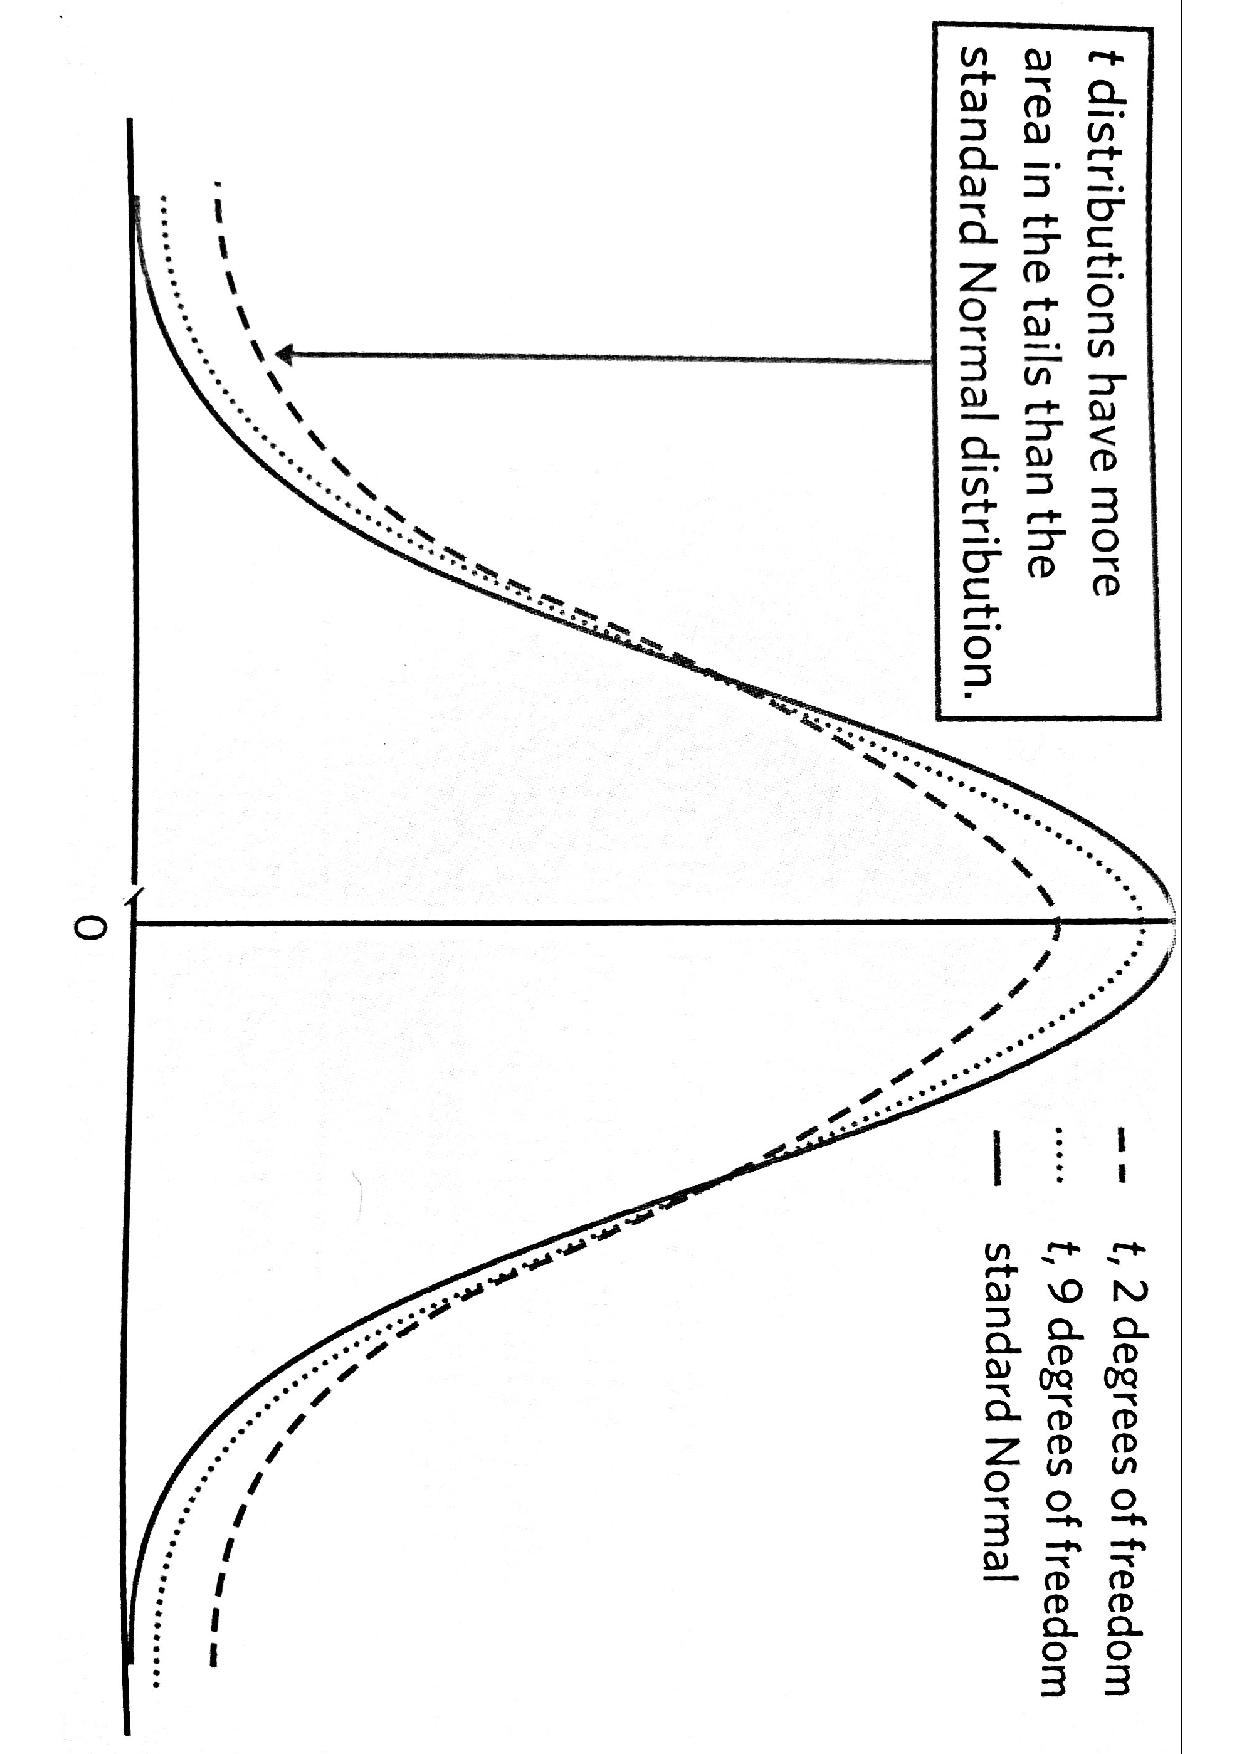
\includegraphics[scale=0.33, angle=90]{t_normal_comparison.pdf}
		\caption{Density curves for the $t$ distribution with 2 and 9 degrees of freedom and for the standard Normal distribution. All are symmetric with center 0. The $t$ distributions are somewhat more spread out.}
	\end{figure}
}

\end{frame}


\begin{frame}[fragile]{$t_{(5)}$ distribution vs. Standard Normal distribution}
\begin{minipage}{0.47\textwidth}
\begin{knitrout}\scriptsize
\definecolor{shadecolor}{rgb}{0.969, 0.969, 0.969}\color{fgcolor}
\begin{alltt}
\hlkwd{library}\hlstd{(mosaic)}
\hlkwd{xqnorm}\hlstd{(}\hlkwc{p} \hlstd{=} \hlkwd{c}\hlstd{(}\hlnum{0.025}\hlstd{,} \hlnum{0.975}\hlstd{))}
\end{alltt}

\end{knitrout}
\begin{knitrout}\scriptsize
\definecolor{shadecolor}{rgb}{0.969, 0.969, 0.969}\color{fgcolor}

{\centering 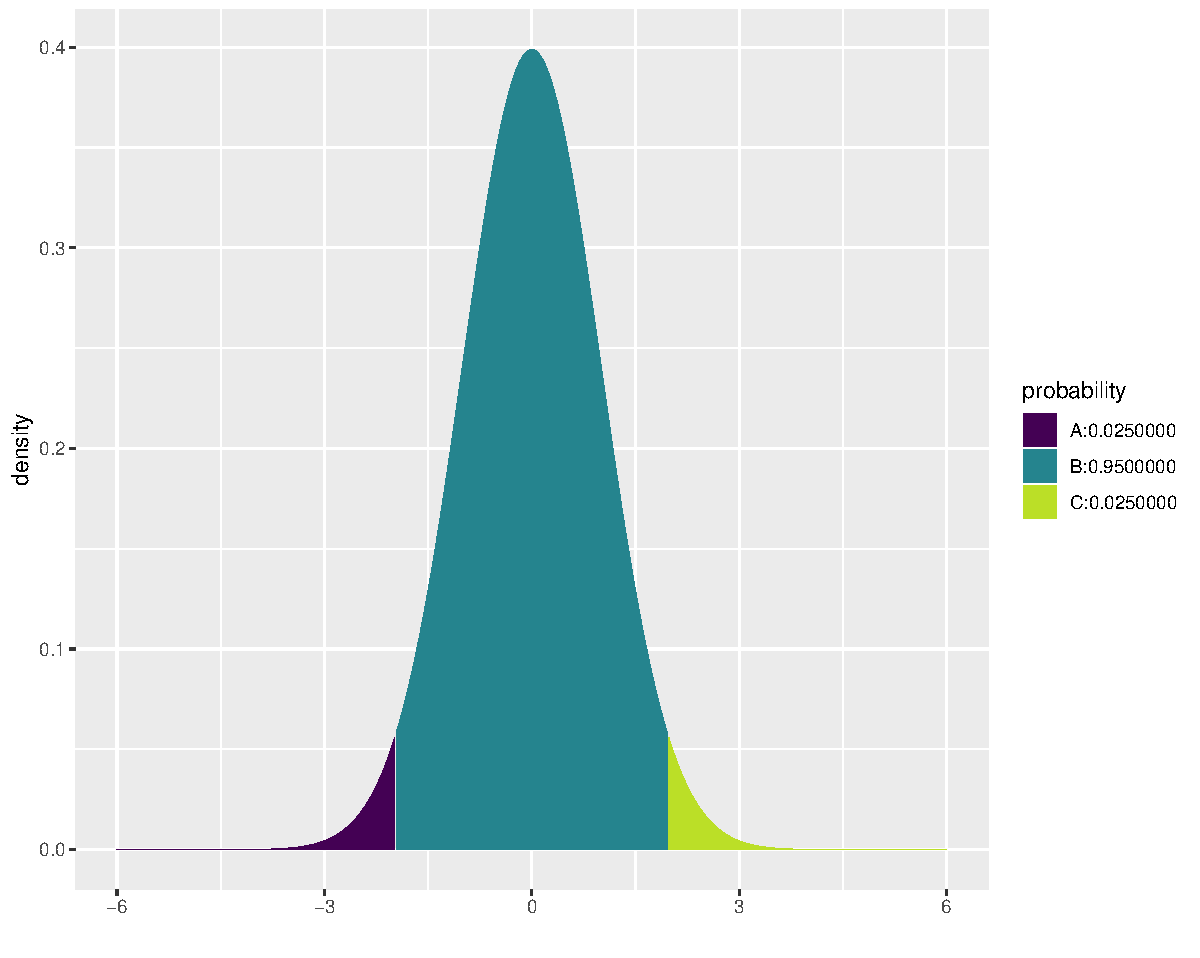
\includegraphics[width=1\linewidth]{figure/unnamed-chunk-2-1} 

}


\begin{verbatim}
## [1] -1.959964  1.959964
\end{verbatim}

\end{knitrout}
\end{minipage}
\begin{minipage}{0.5\textwidth}
\begin{knitrout}\scriptsize
\definecolor{shadecolor}{rgb}{0.969, 0.969, 0.969}\color{fgcolor}
\begin{alltt}
\hlkwd{library}\hlstd{(mosaic)}
\hlkwd{xqt}\hlstd{(}\hlkwc{p} \hlstd{=} \hlkwd{c}\hlstd{(}\hlnum{0.025}\hlstd{,} \hlnum{0.975}\hlstd{),} \hlkwc{df} \hlstd{=} \hlnum{5}\hlstd{)}
\end{alltt}


{\centering 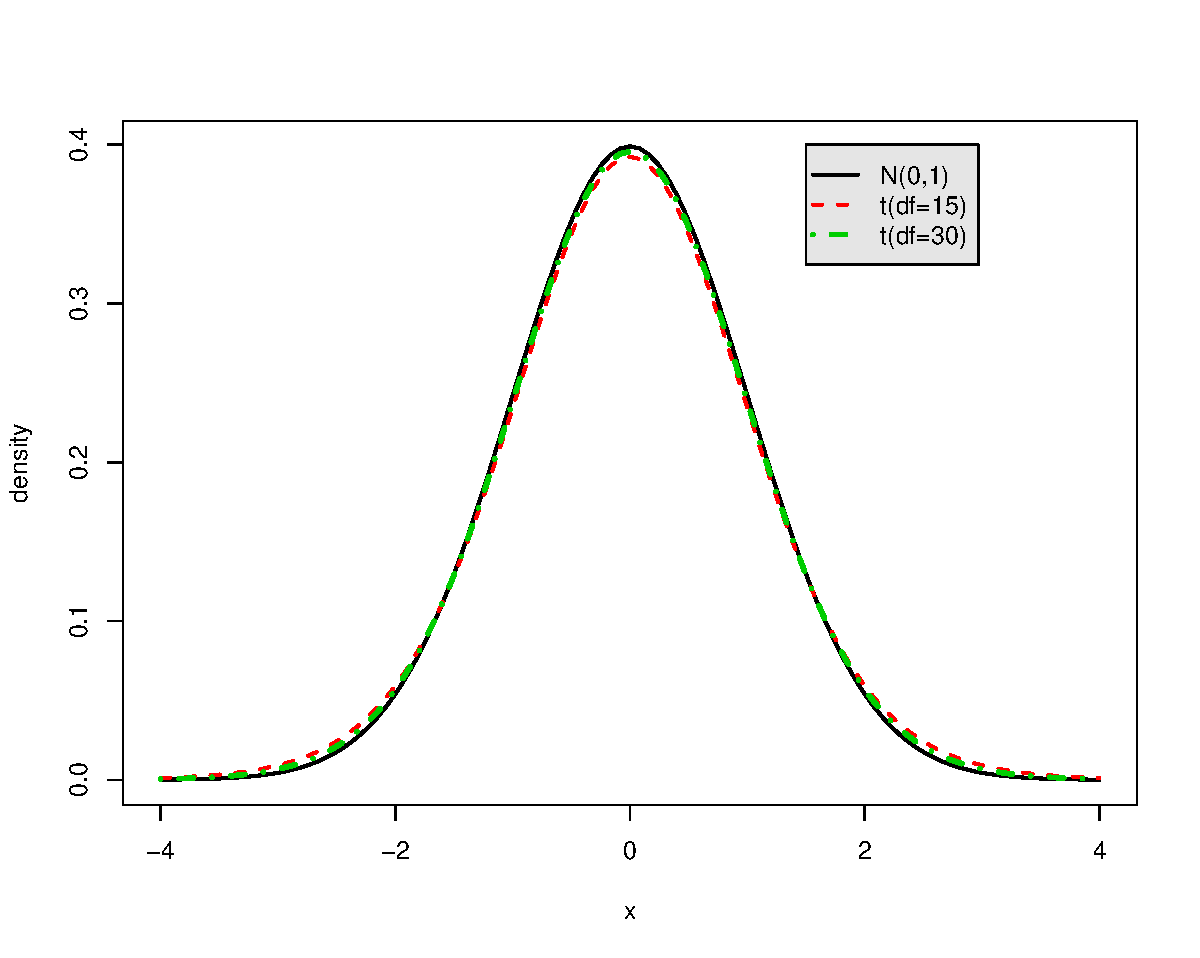
\includegraphics[width=1\linewidth]{figure/unnamed-chunk-3-1} 

}


\begin{verbatim}
## [1] -2.570582  2.570582
\end{verbatim}

\end{knitrout}
\end{minipage}
\end{frame}



\begin{frame}[fragile]{$t_{(30)}$ distribution vs. Standard Normal distribution}
\begin{minipage}{0.47\textwidth}
\begin{knitrout}\scriptsize
\definecolor{shadecolor}{rgb}{0.969, 0.969, 0.969}\color{fgcolor}
\begin{alltt}
\hlkwd{library}\hlstd{(mosaic)}
\hlkwd{xqnorm}\hlstd{(}\hlkwc{p} \hlstd{=} \hlkwd{c}\hlstd{(}\hlnum{0.025}\hlstd{,} \hlnum{0.975}\hlstd{))}
\end{alltt}

\end{knitrout}
\begin{knitrout}\scriptsize
\definecolor{shadecolor}{rgb}{0.969, 0.969, 0.969}\color{fgcolor}

{\centering 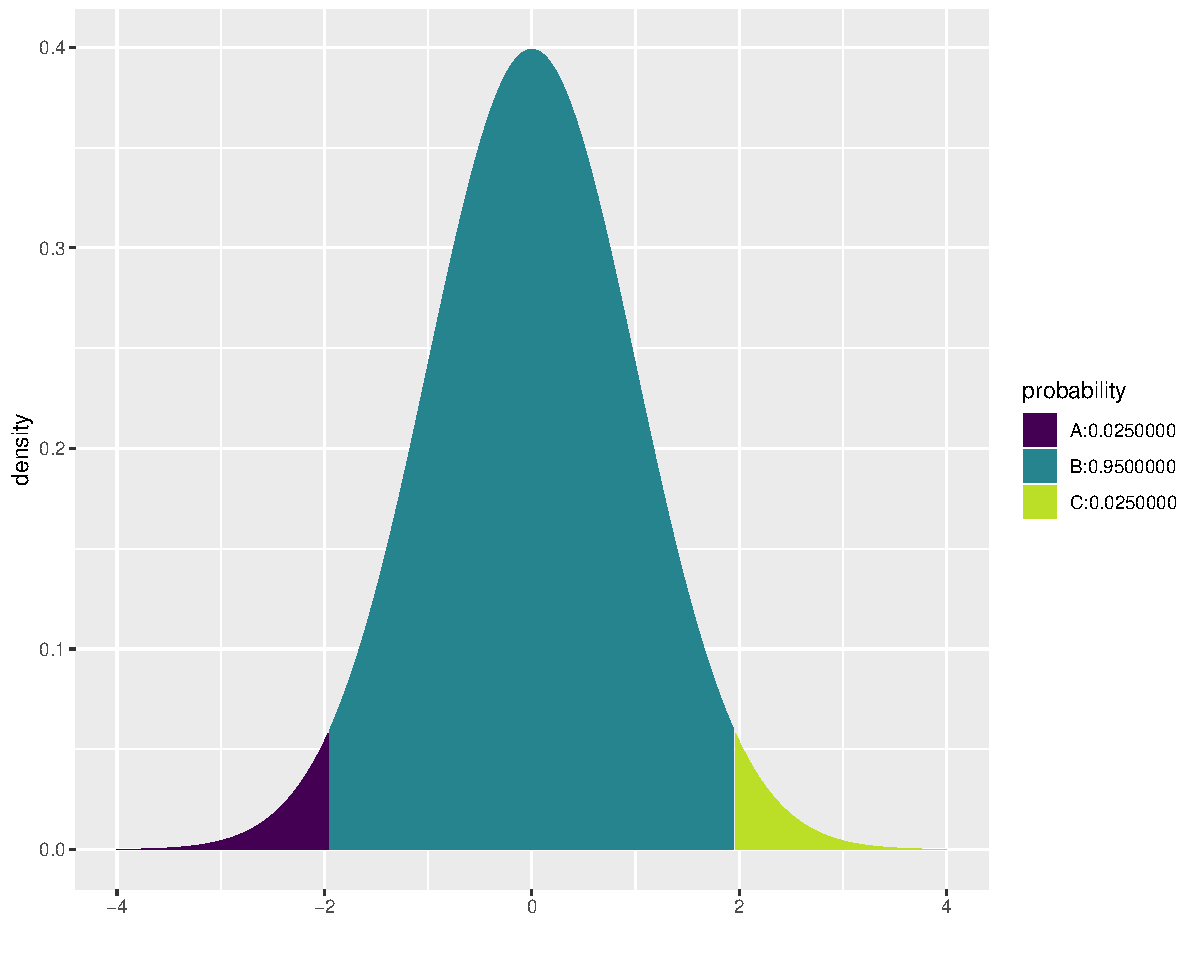
\includegraphics[width=1\linewidth]{figure/unnamed-chunk-5-1} 

}


\begin{verbatim}
## [1] -1.959964  1.959964
\end{verbatim}

\end{knitrout}
\end{minipage}
\begin{minipage}{0.5\textwidth}
\begin{knitrout}\scriptsize
\definecolor{shadecolor}{rgb}{0.969, 0.969, 0.969}\color{fgcolor}
\begin{alltt}
\hlkwd{library}\hlstd{(mosaic)}
\hlkwd{xqt}\hlstd{(}\hlkwc{p} \hlstd{=} \hlkwd{c}\hlstd{(}\hlnum{0.025}\hlstd{,} \hlnum{0.975}\hlstd{),} \hlkwc{df} \hlstd{=} \hlnum{30}\hlstd{)}
\end{alltt}

\end{knitrout}
\begin{knitrout}\scriptsize
\definecolor{shadecolor}{rgb}{0.969, 0.969, 0.969}\color{fgcolor}

{\centering 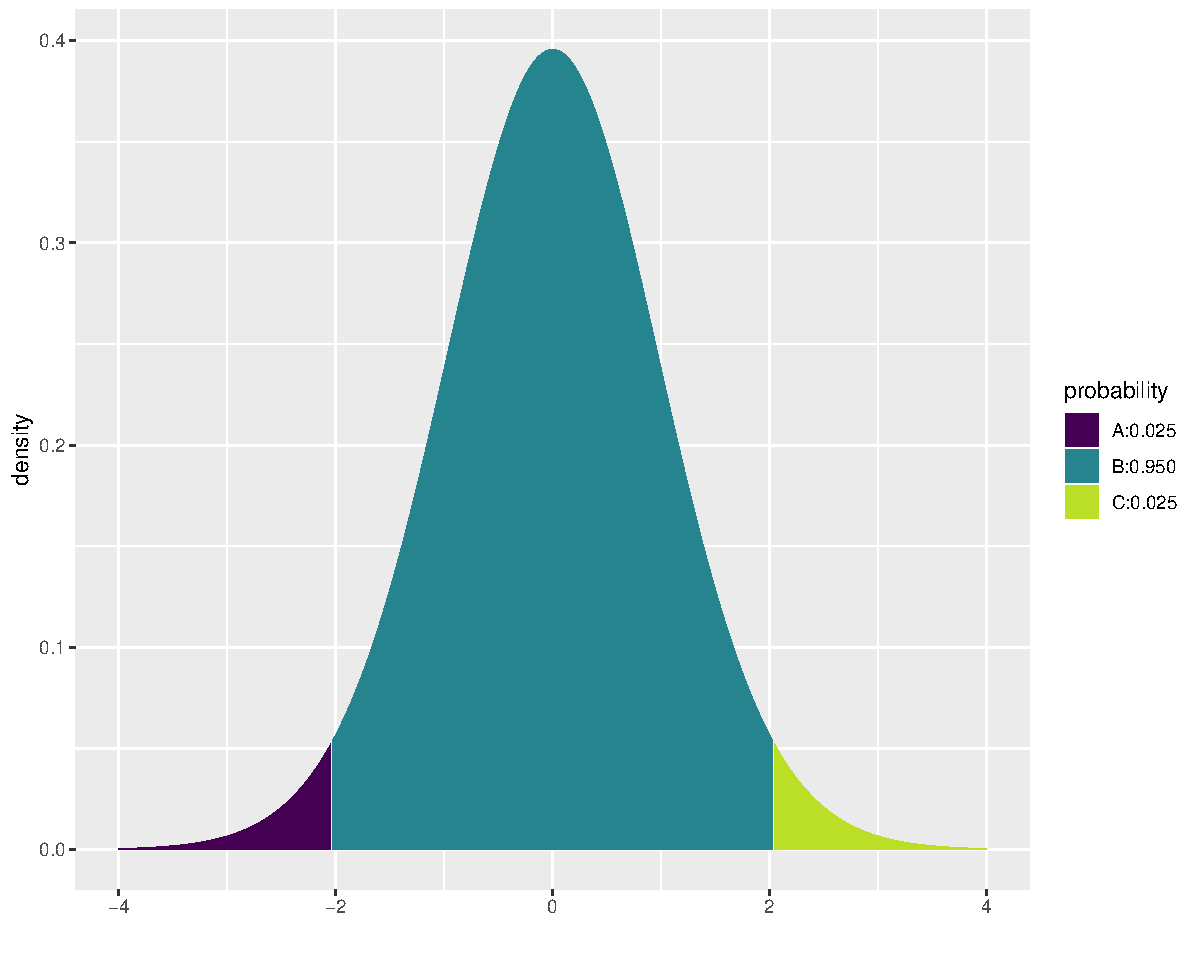
\includegraphics[width=1\linewidth]{figure/unnamed-chunk-7-1} 

}


\begin{verbatim}
## [1] -2.042272  2.042272
\end{verbatim}

\end{knitrout}
\end{minipage}
\end{frame}

%\frame{\frametitle{$t$ distributions}
%	\begin{figure}
%		\begin{center}
%			\epsfig{figure=Tables/psls_table_C.eps,scale=.35}
%		\end{center}
%	\end{figure}
%}


\begin{frame}{$t$ distributions}
\begin{itemize}
	\small
	\item Is symmetric around 0 ( just like the $\mathcal{N}(0,1)$ )
	\item Has a shape like that of the Z distribution, but with a SD slightly larger than
	unity i.e. slightly flatter and heavier-tailed
	\item Shape becomes indistinguishable from Z distribution as $n \rightarrow \infty$ (in fact as $n$ goes much beyond 30)
	\item Instead of  $\pm 1.96 \times  $ SEM for 95\% confidence (or to use as the critical value in a null-hypothesis test), we need these multiples (or critical values): \\ \ \\
	
	\begin{tabular}{r r r r}
		$n$ & `degrees of freedom' & Multiple & from \texttt{R} \\ 
		\hline
		2 & 1 & 12.71 & \texttt{qt(0.975,  1)} \\
		3 & 2 & 4.30 & \texttt{qt(0.975,  2)}\\
		4 & 3 & 3.18 & \texttt{qt(0.975,  3)}\\
		11 &10 & 2.23 & \texttt{qt(0.975, 10)}  \\
		21 & 20 & 2.09 & \texttt{qt(0.975, 20)} \\
		31 & 30 & 2.04 & \texttt{qt(0.975, 30)} \\
		121 & 120 & 1.98 & \texttt{qt(0.975,120)} \\
		$\infty$ & $\infty$ & 1.96 & \texttt{qt(0.975,Inf)}   \\
	\end{tabular}
	
\end{itemize}
\end{frame}

 

\begin{frame}[fragile]{$t$ distributions}
Sample size increases $\rightarrow$ degrees of freedom increase $\rightarrow$ $t$ starts to look like $\mathcal{N}(0,1)$
\begin{knitrout}\scriptsize
\definecolor{shadecolor}{rgb}{0.969, 0.969, 0.969}\color{fgcolor}

{\centering 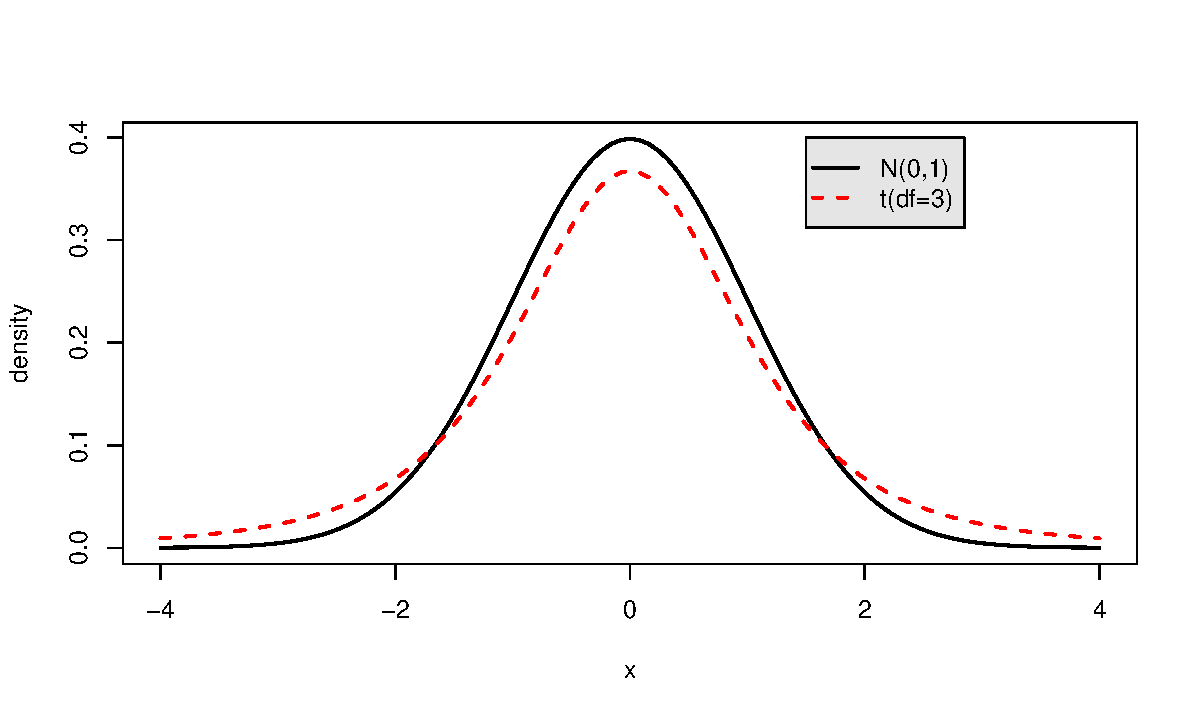
\includegraphics[width=1\linewidth]{figure/unnamed-chunk-8-1} 

}



\end{knitrout}
\end{frame}

\begin{frame}[fragile]{$t$ distributions}
Sample size increases $\rightarrow$ degrees of freedom increase $\rightarrow$ $t$ starts to look like $\mathcal{N}(0,1)$
\begin{knitrout}\scriptsize
\definecolor{shadecolor}{rgb}{0.969, 0.969, 0.969}\color{fgcolor}

{\centering 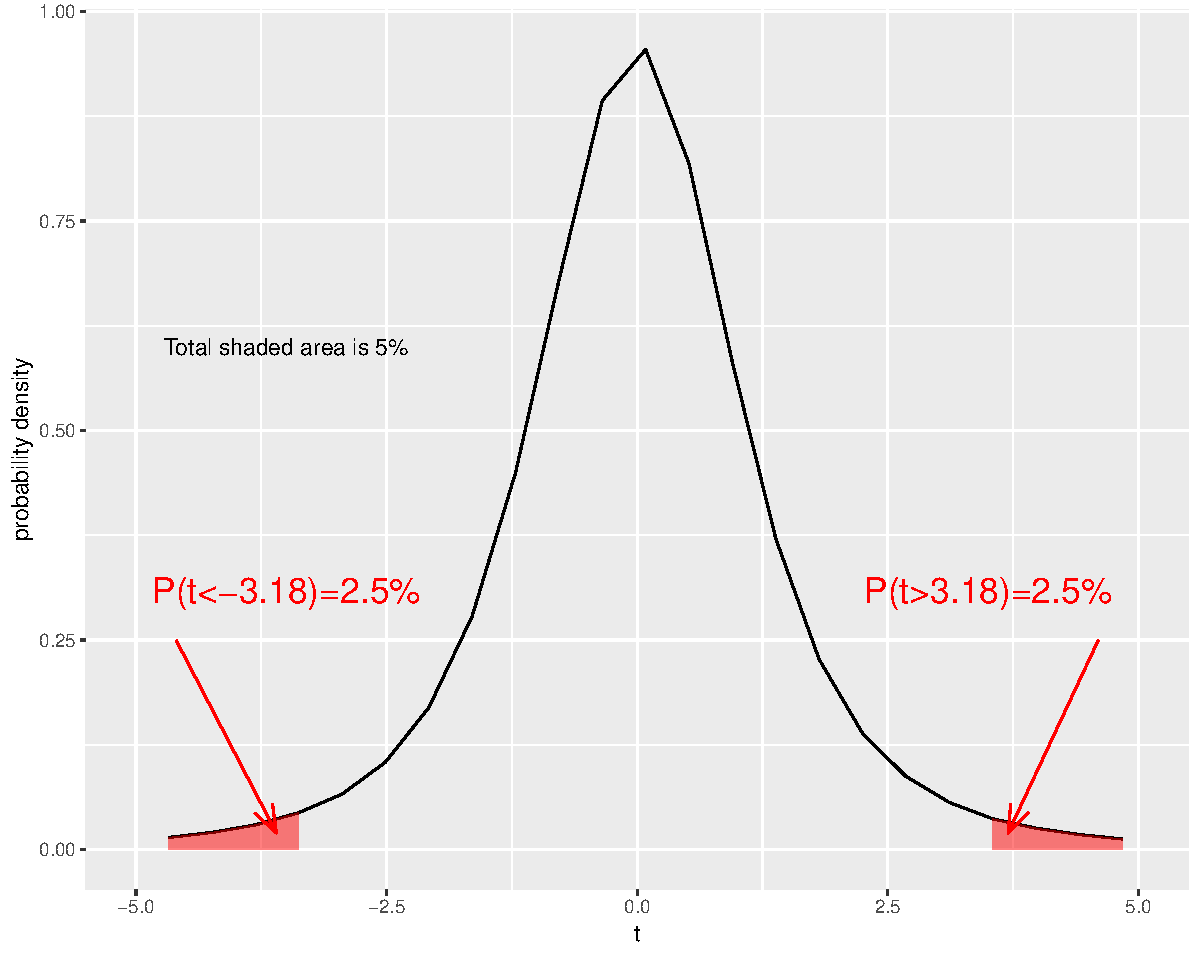
\includegraphics[width=1\linewidth]{figure/unnamed-chunk-9-1} 

}



\end{knitrout}

\Large This is where the infamous $n=30$ comes from !!
\end{frame}

\frame{\frametitle{$t$ procedures} We can calculate CIs and
	perform significance tests much as before (example coming up
	soon).\\\ \\
	
	A significance test of a single sample mean using the $t$-statistic
	is called a \textcolor{blue}{one-sample $t$-test}. \\ \ \\
	
	Collectively, the significance tests and confidence-interval based
	tests using the $t$ distribution are called \underline{$t$ procedures}.  \\ \ \\
	
}

\begin{frame}{The one-sample $t$ test}

\Wider[4em]{
	\centering
		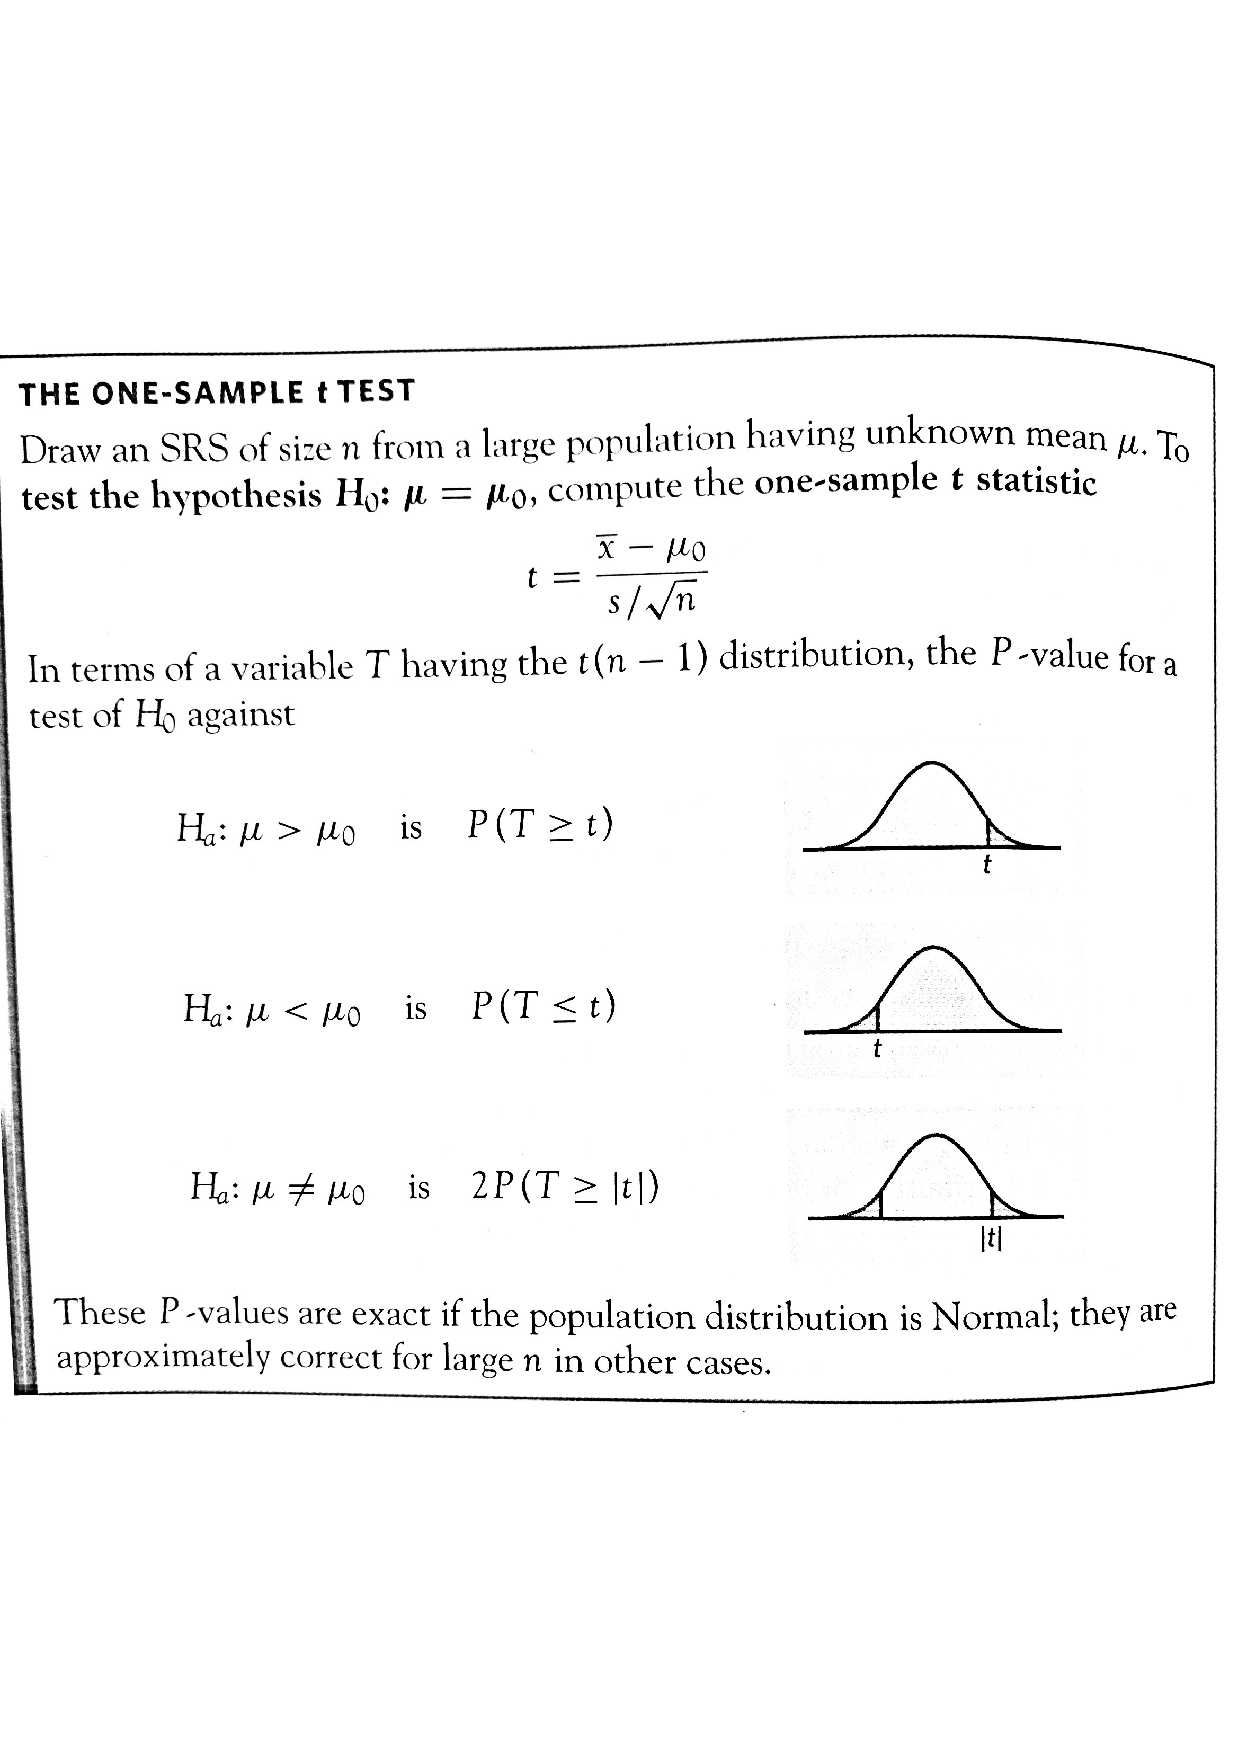
\includegraphics[scale=0.35]{ttest.pdf}
	
}

\end{frame}

 
\begin{frame}{A note about the conditions for $t$ procedures}

\begin{itemize}
	\setlength\itemsep{1em}
	\item B\&M stress that the \textbf{first} of their conditions as \textit{very important}: \textit{we can regard} our data as a simple random sample (SRS) from  the population \pause 
	\item The \textbf{second}, observations from the population have a \textit{\underline{Normal}} distribution with unknown mean parameter $\mu$ and unknown standard deviation parameter $\sigma$ less so 
	\item \textit{In practice}, inference procedures \textit{can accommodate some deviations from
		the Normality condition} when the sample is large enough. 
\end{itemize}
\end{frame}


\frame{\frametitle{Robustness of the $t$ procedures} A statistical
	procedure is said to be \textbf{robust} if it is insensitive to
	violations of the assumptions made. \\ \ \\
	\begin{itemize}
			\setlength\itemsep{1em}
		%\item Results of $t$ procedures (CIs, significance tests) are exact if the
		%population from which the simple random sample was drawn is Normal. \pause
		\item $t$ procedures are not robust against \textit{extreme}
		skewness, \underline{in small samples}, since the procedures are
		based on using $\overline{y}$ and $s$ (which are sensitive to
		outliers).
		\item Recall: \textcolor{blue}{Unless there is a very compelling reason
			(e.g.~known/confirmed error in the recorded data), outliers should not be discarded.}
		
	\end{itemize}
} \frame{\frametitle{Robustness of the $t$ procedures}
	\begin{itemize}
					\setlength\itemsep{2em}
		\item $t$ procedures \textbf{are} robust against other forms
		of non-normality and, even with considerable skew, perform well when $n$ is large. Why?
		\pause
		\item When $n$ is large, $s$ is a good estimate of $\sigma$
		(recall that $s$ is unbiased and, like most estimates, precision
		improves with increasing sample size) \pause
		\item CLT: $\overline{y}$ will be Normal when $n$ is large, even if the
		population data are not


	\end{itemize}
}



\begin{frame}{When and why we use the $t$-distribution}
\mylist{When $\sigma$ is unknown use $t$ distribution. \blue{but why?}; \pause the spread of the $t$ distribution is greater than $\mathcal{N}(0,1)$  }
\end{frame}



\begin{frame}[fragile]{Rejecting the Null ($H_0: \mu = \mu_0$) when $\sigma$ is known}
\small
\[ \underbrace{z_{0.975}}_{\textrm{critical value}}=1.96 = \frac{\bar{y}-\mu_0}{\sigma/\sqrt{n}} \rightarrow \frac{1.96 }{\sqrt{n}}\sigma = \bar{y}-\mu_0   \] which means that to reject $H_0$ the difference between your sample mean and $\mu_0$ needs to be \blue{greater than $\frac{1.96}{\sqrt{n}}$ standard deviations} 

\begin{knitrout}\scriptsize
\definecolor{shadecolor}{rgb}{0.969, 0.969, 0.969}\color{fgcolor}
\begin{alltt}
\hlstd{mosaic}\hlopt{::}\hlkwd{xqnorm}\hlstd{(}\hlkwc{p} \hlstd{=} \hlkwd{c}\hlstd{(}\hlnum{0.025}\hlstd{,} \hlnum{0.975}\hlstd{))}
\end{alltt}


{\centering 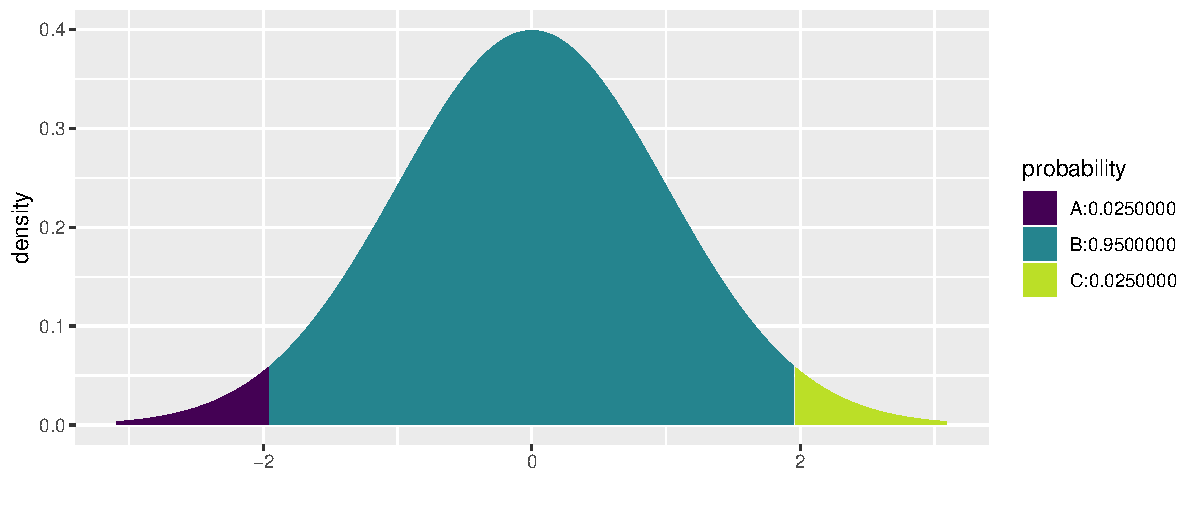
\includegraphics[width=1\linewidth]{figure/unnamed-chunk-11-1} 

}


\begin{verbatim}
## [1] -1.959964  1.959964
\end{verbatim}

\end{knitrout}
\end{frame}



\begin{frame}[fragile]{Rejecting the Null ($H_0: \mu = \mu_0$) when $\sigma$ is unknown}
\small
\[ \underbrace{t_{0.975,df=3}^\star}_{\textrm{critical value}}=3.18 = \frac{\bar{y}-\mu_0}{s/\sqrt{n}} \rightarrow  \frac{3.18}{\sqrt{n}}s = \bar{y}-\mu_0   \] which means that to reject $H_0$ the difference between your sample mean and $\mu_0$ needs to be \blue{greater than $\frac{3.18}{\sqrt{n}}$ standard deviations} 


\begin{knitrout}\scriptsize
\definecolor{shadecolor}{rgb}{0.969, 0.969, 0.969}\color{fgcolor}
\begin{alltt}
\hlstd{mosaic}\hlopt{::}\hlkwd{xqt}\hlstd{(}\hlkwc{p} \hlstd{=} \hlkwd{c}\hlstd{(}\hlnum{0.025}\hlstd{,} \hlnum{0.975}\hlstd{),} \hlkwc{df} \hlstd{=} \hlnum{3}\hlstd{)}
\end{alltt}


{\centering 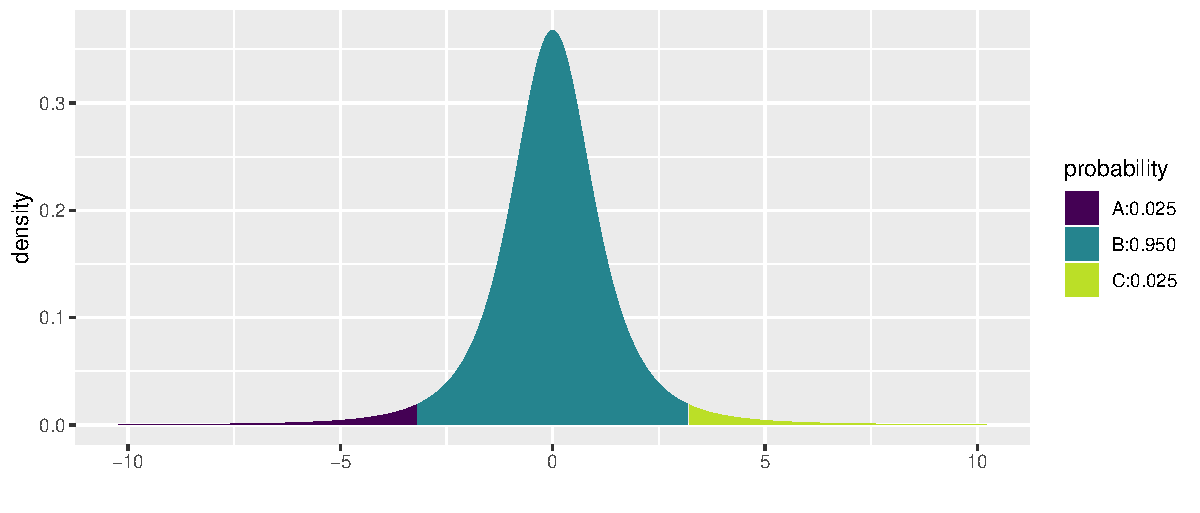
\includegraphics[width=1\linewidth]{figure/unnamed-chunk-13-1} 

}


\begin{verbatim}
## [1] -3.182446  3.182446
\end{verbatim}

\end{knitrout}

\end{frame}




\begin{frame}{Summary of $t$ distribution}
\mylist{Its harder to reject the null when using the $t$ distribution; \pause Confidence intervals are also wider; \pause This is due to our uncertainty about the estimated variance ;\pause Larger samples lead to more accurate estimates of $\sigma$; \pause This is reflected in the fact that there is a different $t$ distribution for each sample size  ; \pause As $n \rightarrow \infty$, sample standard deviation $s$ gets closer to $\sigma$; \pause As degrees of freedom increase, $t$ distribution gets closer to Normal distribution}
\end{frame}


\section{Examples}


\begin{frame}{Application: How fast is your reaction time?}
\small\url{https://faculty.washington.edu/chudler/java/redgreen.html} 

\framedgraphic{JHReactionTimes.png}

\end{frame}


\begin{frame}[fragile]{Application: How fast is your reaction time?}
\begin{knitrout}\scriptsize
\definecolor{shadecolor}{rgb}{0.969, 0.969, 0.969}\color{fgcolor}
\begin{alltt}
\hlstd{reaction.times} \hlkwb{<-} \hlkwd{c}\hlstd{(}\hlnum{325}\hlstd{,}\hlnum{327}\hlstd{,}\hlnum{357}\hlstd{,}\hlnum{299}\hlstd{,}\hlnum{378}\hlstd{)}\hlopt{/}\hlnum{1000}
\hlkwd{summary}\hlstd{(reaction.times)}
\end{alltt}
\begin{verbatim}
##    Min. 1st Qu.  Median    Mean 3rd Qu.    Max. 
##  0.2990  0.3250  0.3270  0.3372  0.3570  0.3780
\end{verbatim}
\begin{alltt}
\hlkwd{round}\hlstd{(}\hlkwd{sd}\hlstd{(reaction.times),}\hlnum{3}\hlstd{)}
\end{alltt}
\begin{verbatim}
## [1] 0.031
\end{verbatim}
\begin{alltt}
\hlkwd{length}\hlstd{(reaction.times)}
\end{alltt}
\begin{verbatim}
## [1] 5
\end{verbatim}

\end{knitrout}

\end{frame}


\begin{frame}[fragile]{5 ways of calculating a confidence interval}

We are interested in calculating a 95\% confidence interval for the mean reaction time based on the sample of 5 reaction times. \\ \ \\
\pause
Four ways of doing this:
\begin{enumerate}
	\setlength\itemsep{1em}
	\item By hand (using the $\pm$ formula and \texttt{R} as a calculator)
	\item Using the quantile function for the $t$ distribution \texttt{stats::qt}
	\item Fitting an intercept-only regression model ($y = \beta_0 + \varepsilon$)
	\item Using a canned function (\texttt{mosaic::t.test}, \texttt{stats::t.test})
	\item Bootstrap
\end{enumerate}

\end{frame}

\begin{frame}[fragile]{1. By hand using the $\pm$ formula}
\begin{knitrout}\scriptsize
\definecolor{shadecolor}{rgb}{0.969, 0.969, 0.969}\color{fgcolor}
\begin{alltt}
\hlstd{n} \hlkwb{<-} \hlkwd{length}\hlstd{(reaction.times)}
\hlstd{SEM} \hlkwb{<-} \hlkwd{sd}\hlstd{(reaction.times)}\hlopt{/}\hlkwd{sqrt}\hlstd{(n)}
\end{alltt}
\begin{verbatim}
## [1] 0.01372734
\end{verbatim}
\begin{alltt}
\hlstd{ybar} \hlkwb{<-} \hlkwd{mean}\hlstd{(reaction.times)}
\end{alltt}
\begin{verbatim}
## [1] 0.3372
\end{verbatim}
\begin{alltt}
\hlstd{multiple.for.95pct} \hlkwb{<-} \hlstd{stats}\hlopt{::}\hlkwd{qt}\hlstd{(}\hlkwc{p} \hlstd{=} \hlkwd{c}\hlstd{(}\hlnum{0.025}\hlstd{,} \hlnum{0.975}\hlstd{),} \hlkwc{df} \hlstd{= n}\hlopt{-}\hlnum{1}\hlstd{)}
\end{alltt}
\begin{verbatim}
## [1] -2.776445  2.776445
\end{verbatim}
\begin{alltt}
\hlstd{by_hand_CI} \hlkwb{<-} \hlstd{ybar} \hlopt{+} \hlstd{multiple.for.95pct} \hlopt{*} \hlstd{SEM}
\end{alltt}
\begin{verbatim}
## [1] 0.29909 0.37531
\end{verbatim}

\end{knitrout}
\end{frame}

\begin{frame}[fragile]{2. Using \texttt{stats::qt}}
\textit{Note: \texttt{R} only provides the standard $t$ distribution. In order to get a scaled version we must define our own function.}

\vspace*{0.2in}

\begin{knitrout}\scriptsize
\definecolor{shadecolor}{rgb}{0.969, 0.969, 0.969}\color{fgcolor}
\begin{alltt}
\hlstd{n} \hlkwb{<-} \hlkwd{length}\hlstd{(reaction.times)}
\hlstd{SEM} \hlkwb{<-} \hlkwd{sd}\hlstd{(reaction.times)}\hlopt{/}\hlkwd{sqrt}\hlstd{(n)}
\hlstd{ybar} \hlkwb{<-} \hlkwd{mean}\hlstd{(reaction.times)}

\hlcom{# scaled version of the standard t distribution}
\hlstd{qt_ls} \hlkwb{<-} \hlkwa{function}\hlstd{(}\hlkwc{p}\hlstd{,} \hlkwc{df}\hlstd{,} \hlkwc{mean}\hlstd{,} \hlkwc{sd}\hlstd{)} \hlkwd{qt}\hlstd{(}\hlkwc{p} \hlstd{= p,} \hlkwc{df} \hlstd{= df)} \hlopt{*} \hlstd{sd} \hlopt{+} \hlstd{mean}

\hlkwd{qt_ls}\hlstd{(}\hlkwc{p} \hlstd{=} \hlkwd{c}\hlstd{(}\hlnum{0.025}\hlstd{,} \hlnum{0.975}\hlstd{),} \hlkwc{df} \hlstd{= n} \hlopt{-} \hlnum{1}\hlstd{,} \hlkwc{mean} \hlstd{= ybar,} \hlkwc{sd} \hlstd{= SEM)}
\end{alltt}
\begin{verbatim}
## [1] 0.2990868 0.3753132
\end{verbatim}

\end{knitrout}
\end{frame}


\begin{frame}[fragile]{3. Fitting an intercept-only regression model}
\begin{knitrout}\scriptsize
\definecolor{shadecolor}{rgb}{0.969, 0.969, 0.969}\color{fgcolor}
\begin{alltt}
\hlstd{fit} \hlkwb{<-} \hlstd{stats}\hlopt{::}\hlkwd{lm}\hlstd{(reaction.times} \hlopt{~} \hlnum{1}\hlstd{)}
\hlkwd{summary}\hlstd{(fit)}
\end{alltt}
\begin{verbatim}
## 
## Call:
## stats::lm(formula = reaction.times ~ 1)
## 
## Residuals:
##       1       2       3       4       5 
## -0.0122 -0.0102  0.0198 -0.0382  0.0408 
## 
## Coefficients:
##             Estimate Std. Error t value Pr(>|t|)    
## (Intercept)  0.33720    0.01373   24.56 1.63e-05 ***
## ---
## Signif. codes:  0 '***' 0.001 '**' 0.01 '*' 0.05 '.' 0.1 ' ' 1
## 
## Residual standard error: 0.0307 on 4 degrees of freedom
\end{verbatim}
\begin{alltt}
\hlstd{stats}\hlopt{::}\hlkwd{confint}\hlstd{(fit)}
\end{alltt}
\begin{verbatim}
##                 2.5 %    97.5 %
## (Intercept) 0.2990868 0.3753132
\end{verbatim}

\end{knitrout}
\end{frame}


\begin{frame}[fragile]{3. Fitting an intercept-only regression model}
In the regression output:
\begin{itemize}
	\setlength\itemsep{1em}
	\item \texttt{Estimate}: the mean reaction time (an estimate of the intercept $\beta_0$)
	\item \texttt{t value}: the test statistic 
	\item \texttt{Std. Error}: the standard error of the mean (SEM)
	\item \texttt{Pr(>|t|)}: is the $p$-value
\end{itemize} 


\end{frame}


\begin{frame}[fragile]{3. Fitting an intercept-only regression model}



\small
These are based on the (useless) null hypothesis $H_0: \mu_0 = 0$ \\ \ \\

\begin{itemize}
	\item \texttt{t value} = $\frac{\bar{y} - \mu_0}{s / \sqrt{n}}$ = $\frac{0.33720 - 0}{0.01373}$ = 24.56
	\item \texttt{Pr(>|t|)} \\ \ \\
	= $P(\textrm{t value} > t_{(n-1)}) + P(-\textrm{t value} < t_{(n-1)})$ \\ \ \\
	 = \small{\texttt{pt(q = 24.56, df = n-1, lower.tail = FALSE)} +  \texttt{pt(q = -24.56, df = n-1)}} \\ \ \\
	  = \ensuremath{8.1549827\times 10^{-6}} + \ensuremath{8.1549827\times 10^{-6}} = \ensuremath{1.6309965\times 10^{-5}}
\end{itemize}


\end{frame}



\begin{frame}[fragile]{4. Canned function}

\begin{knitrout}\scriptsize
\definecolor{shadecolor}{rgb}{0.969, 0.969, 0.969}\color{fgcolor}
\begin{alltt}
\hlstd{stats}\hlopt{::}\hlkwd{t.test}\hlstd{(reaction.times)}
\end{alltt}
\begin{verbatim}
## 
## 	One Sample t-test
## 
## data:  reaction.times
## t = 20, df = 4, p-value = 2e-05
## alternative hypothesis: true mean is not equal to 0
## 95 percent confidence interval:
##  0.299 0.375
## sample estimates:
## mean of x 
##     0.337
\end{verbatim}

\end{knitrout}

\end{frame}



\begin{frame}[fragile]{5. Bootstrap}

\begin{knitrout}\scriptsize
\definecolor{shadecolor}{rgb}{0.969, 0.969, 0.969}\color{fgcolor}
\begin{alltt}
\hlstd{df_react} \hlkwb{<-} \hlkwd{data.frame}\hlstd{(reaction.times)} \hlcom{# need data.frame to bootstrap}
\hlstd{s_dist} \hlkwb{<-} \hlkwd{do}\hlstd{(}\hlnum{10000}\hlstd{)} \hlopt{*} \hlkwd{mean}\hlstd{(} \hlopt{~} \hlstd{reaction.times,}
                \hlkwc{data} \hlstd{=} \hlkwd{resample}\hlstd{(df_react))}
\hlstd{CI_95} \hlkwb{<-} \hlkwd{quantile}\hlstd{(}\hlopt{~} \hlstd{mean,} \hlkwc{data} \hlstd{= s_dist,} \hlkwc{probs} \hlstd{=} \hlkwd{c}\hlstd{(}\hlnum{0.025}\hlstd{,} \hlnum{0.975}\hlstd{))}
\end{alltt}
\begin{verbatim}
##  2.5% 97.5% 
## 0.315 0.362
\end{verbatim}


{\centering 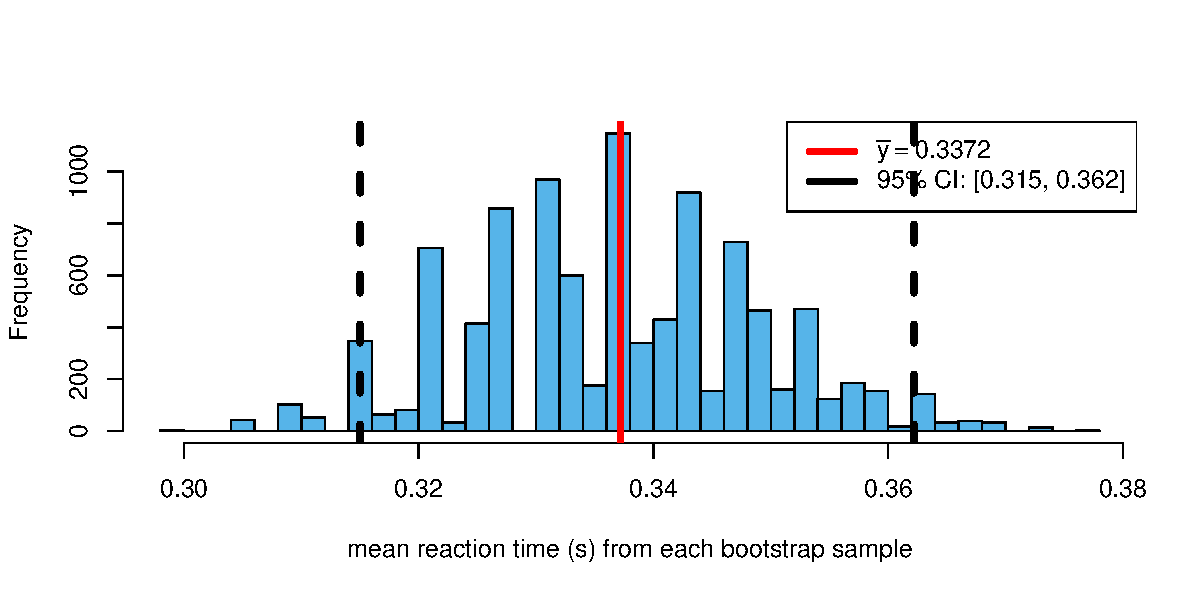
\includegraphics[width=1\linewidth]{figure/unnamed-chunk-20-1} 

}



\end{knitrout}

\end{frame}




\end{document}






